\documentclass[12pt,a4paper]{article}
\usepackage[lmargin=3cm, tmargin=3cm, rmargin=2cm, bmargin=2cm]{geometry}
\usepackage{sbc-template}
\usepackage{graphicx,url}
\usepackage[utf8]{inputenc}  
\usepackage{ragged2e}
\usepackage{setspace}
\onehalfspacing
\setlength{\parindent}{1.25cm}
\usepackage{indentfirst}
\usepackage{graphicx}
\usepackage{float}
\usepackage{url}
\usepackage[brazil]{babel}
\usepackage{hyperref}
\usepackage[numbers]{natbib}
\usepackage{titlesec}
\usepackage{tocloft}
\usepackage{appendix}
\usepackage{titlesec}
\usepackage{acronym}
\usepackage[xindy,style=long]{glossaries} 
\usepackage{chngcntr}
\usepackage{fancyhdr}

\newglossaryentry{CTP Acolhe}{
                name={CTP Acolhe},
                sort={CTP Acolhe:},
                description={Nome do projeto e sistema. - Citado em:}
                }

\newglossaryentry{CTP}{
                name={CTP},
                sort= {CTP:},
                description={Nome do projeto e sistema. - Citado em:}
                }

\newglossaryentry{Sistema Web}{
                name={Sistema Web},
                sort={Sistema Web:},
                description={É um software hospedado na internet. - Citado em:}
                }
                
\newglossaryentry{MySQL}{
                name={MySQL},
                sort={MySQL:},
                description={É um sistema de gerenciamento de banco de dados, que utiliza a linguagem SQL como interface. - Citado em:}
                }

\newglossaryentry{SQL}{
                name={SQL},
                sort={SQL:},
                description={Linguagem de consulta estruturada. - Citado em:}
                }

\newglossaryentry{Oracle}{
                name={Oracle},
                sort={Oracle:},
                description={A Oracle Corporation é uma empresa multinacional de tecnologia e informática norte-americana, especializada no desenvolvimento e comercialização de hardware e softwares e de banco de dados. - Citado em:}
                }
                
\newglossaryentry{Sony}{
                name={Sony},
                sort={Sony:},
                description={Group Corporation é uma marca criadora e fabricadora de aparelhos eletronicos. - Citado em:}
                }

\newglossaryentry{Bradesco}{
                name={Bradesco},
                sort={Bradesco:},
                description={É um banco brasileiro. - Citado em:}
                }

\newglossaryentry{NASA}{
                name={NASA},
                sort={NASA:},
                description={Administração Nacional da Aeronáutica e Espaço é uma agência do governo federal dos Estados Unidos responsável pela pesquisa e desenvolvimento de tecnologias e programas de exploração espacial. - Citado em:}
                }

\newglossaryentry{C}{
                name={C},
                sort={C:},
                description={Linguagem de programação. - Citado em:}
                }

\newglossaryentry{C++}{
                name={C++},
                sort={C++:},
                description={Linguagem de programação. - Citado em:}
                }

\newglossaryentry{Windows}{
                name={Windows},
                sort={Windows:},
                description={É um sistema operacional de interface gráfica multitarefa. - Citado em:}
                }

\newglossaryentry{Linux}{
                name={Linux},
                sort={Linux:},
                description={É um sistema operacional. - Citado em:}
                }

\newglossaryentry{Java}{
                name={Java},
                sort={Java:},
                description={É uma linguagem de programação orientada a objetos . - Citado em:}
                }

\newglossaryentry{JavaScript}{
                name={JavaScript},
                sort={JavaScript:},
                description={É uma linguagem de programação estruturada . - Citado em:}
                }

\newglossaryentry{Mac OS X Server}{
                name={Mac OS X Server},
                sort={Mac OS X Server:},
                description={É um sistema operacional. - Citado em:}
                }

\newglossaryentry{Scrum}{
                name={Scrum},
                sort={Scrum:},
                description={É uma estrutura para gerenciamento de projetos. - Citado em:}
                }

\newglossaryentry{Sprints}{
                name={Sprints},
                sort={Sprints:},
                description={Cada um dos per ́ıodos utilizados para a conclus ̃ao de uma parte do projeto. - Citado em:}
                }
                
\newglossaryentry{Stakeholders}{
                name={Stakeholders},
                sort={Stakeholders:},
                description={Pessoas, grupos que possuem um nível de interesse em atividades  de uma determinada organização. - Citado em:}
                }

\newglossaryentry{Time-Boxed}{
                name={Time-Boxed},
                sort={Time-Boxed:},
                description={O tempo de duração para realizar uma determinada tarefa. - Citado em:}
                }

\newglossaryentry{Trello}{
                name={Trello},
                sort={Trello:},
                description={Ferramenta de Gestão de Projetos. - Citado em:}
                }
                
\newglossaryentry{Kanban}{
                name={Kanban},
                sort={Kanban:},
                description={Método popular de gestão de fluxo de trabalho. - Citado em:}
                }

\newglossaryentry{DB-Engines}{
                name={DB-Engines},
                sort={DB-Engines:},
                description={Um ranking que classifica os sistemas de gerenciamento de banco de dados por popularidade. - Citado em:}
                }

\newglossaryentry{StackOverflow}{
                name={StackOverflow},
                sort={StackOverflow:},
                description={Um site de perguntas e respostas na área da programação de computadores. - Citado em:}
                }

\newglossaryentry{FIGMA}{
                name={FIGMA},
                sort={FIGMA:},
                description={Uma plataforma para a contrução de design de interfaces e protótipos. - Citado em:}
                }

\newglossaryentry{FIGMA}{
                name={FIGMA},
                sort={FIGMA:},
                description={Uma plataforma para a contrução de design de interfaces e protótipos. - Citado em:}
                }
    
\newglossaryentry{FreePik}{
                name={FreePik},
                sort={FreePik:},
                description={Um site de banco de imagens. - Citado em:}
                }

\newglossaryentry{Light}{
                name={Light},
                sort={Light:},
                description={Esquemas de cores mais claras para a interface. - Citado em:}
                }

\newglossaryentry{Dark}{
                name={Dark},
                sort={Dark:},
                description={Esquema de cores mais escuras para a interface. - Citado em:}
                }

\newglossaryentry{Software}{
                name={Software},
                sort={Software:},
                description={Uma sequência de instruções escritas para serem interpretadas por um computador para executar tarefas específicas. - Citado em:}
                }

\newglossaryentry{Lotus}{
                name={Lotus},
                sort={Lotus:},
                description={Nome da equipe responsável pela execução do projeto. - Citado em:}
                }

\newglossaryentry{Spring}{
                name={Spring},
                sort={Spring:},
                description={É um framework desenvolvimento para facilitar a criação de aplicações Java utilizando diversos módulos independentes. - Citado em:}
                }

\newglossaryentry{Facebook}{
                name={Facebook},
                sort={Facebook:},
                description={Rede Social. - Citado em:}
                }

\newglossaryentry{Overleaf}{
                name={Overleaf},
                sort={Overleaf:},
                description={É um editor LaTeX colaborativo baseado em nuvem usado para escrever, editar e publicar documentos científicos. - Citado em:}
                }

\newglossaryentry{HTTP}{
                name={HTTP},
                sort={HTTP:},
                description={Protocolo de comunicação utilizado na internet para envio de dados entre um cliente e um servidor. - Citado em:}
                }
                
\newglossaryentry{Git}{
                name={Git},
                sort={Git:},
                description={Sistema de controle de versão distribuído. - Citado em:}
                }

\newglossaryentry{GitHub}{
                name={GitHub},
                sort={GitHub:},
                description={Plataforma de hospedagem, revisão e colaboração de código em desenvolvimento de software. - Citado em:}
                }

\newglossaryentry{REST API}{
                name={REST API},
                sort={REST API:},
                description={Interface de programação de aplicações que segue os princípios de arquitetura REST (Representational State Transfer). Permite a comunicação entre sistemas e a troca de dados padronizada e baseada em recursos.  - Citado em:}
                }

\newglossaryentry{JSON}{
                name={JSON},
                sort={JSON:},
                description={JavaScript Object Notation (JSON) é uma notação de objetos em JavaScript, um formato de troca de dados entre sistemas independentes   - Citado em:}
                }

\newglossaryentry{hard-code}{
                name={hard-code},
                sort={hard-code:},
                description={Código escrito não previsto para alterações, com dados alocados diretamente no código fonte da aplicação. - Citado em:}
                }

\newglossaryentry{Railway}{
                name={Railway},
                sort={Railway:},
                description={Plataforma intuitiva de hospedagem para sistemas e bancos de dados. - Citado em:}
                }

\newglossaryentry{Netlify}{
                name={Netlify},
                sort={Netlify:},
                description={Plataforma de hospedagem com foco em projetos web e desenvolvimento front-end. - Citado em:}
                }

\newglossaryentry{TLS}{
                name={TLS},
                sort={TLS:},
                description={Protocolo de segurança que auxilia na privacidade de dados trafegados na web pelo uso de criptografia na comunicação entre os usuários e a aplicação. - Citado em:}
                }

\newglossaryentry{CDN}{
                name={CDN},
                sort={CDN:},
                description={Rede de distribuição de conteúdo, um grupo de servidores geograficamente distribuídos que armazenam conteúdo em cache próximo aos usuários finaiso. - Citado em:}
                }

\newglossaryentry{Deploy}{
                name={Deploy},
                sort={Deploy:},
                description={Processo de implantação de uma aplicação em um ambiente de produção, tornando-o acessível aos usuários finais. - Citado em:}
                }

\newglossaryentry{branch}{
                name={branch},
                sort={branch:},
                description={Uma ramificação, linha de desenvolvimento independente, que permite que diferentes versões do código coexistam simultaneamente. - Citado em:}
                }

\newglossaryentry{imgBB}{
                name={imgBB},
                sort={imgBB:},
                description={Serviço de hospedagem de imagens que permite aos usuários fazer o upload e interpretar imagens como links. - Citado em:}
                }

\newglossaryentry{API}{
                name={API},
                sort={API:},
                description={Um conjunto de regras e protocolos que permitem a comunicação e interação entre diferentes softwares e serviços. - Citado em:}
                }

\newglossaryentry{Back-end}{
                name={Back-end},
                sort={Back-end:},
                description={Toda a parte da programação voltada ao funcionamento interno de um software. - Citado em:}
                }

\newglossaryentry{Front-end}{
                name={Front-end},
                sort={Front-end:},
                description={É a parte visual e interativa de um software. - Citado em:}
                }

\newglossaryentry{Discord}{
                name={Discord},
                sort={Discord:},
                description={Uma plataforma para as pessoas com interesses semelhantes compartilharem e se comunicarem. - Citado em:}
                }

\usepackage[colorlinks]{hyperref}
\hypersetup{
    colorlinks=true,
    linkcolor=black,
    filecolor=blue,      
    urlcolor=blue,
    pdftitle={Overleaf Example},
    pdfpagemode=FullScreen,
    }
\sloppy

\title{CTP Acolhe}

\author{Isabela C. Silva, Jéssica S. Silva, Kaio Victtor Galvão, Maria Eduarda Lúcio,\\ Matheus S. Portes, Nickolas T. Silva, Werônica A. Melo}

 \address{Instituto Federal de Educação, Ciência e Tecnologia de São Paulo (IFSP)\\
 São Paulo -- SP -- Brasil\\  Curso Técnico em Informática Integrado ao Ensino Médio\\ PDS - Prática para Desenvolvimento de Sistemas}

\renewcommand{\cfttoctitlefont}{\large\bfseries}

\titleformat{\section}[block]{\justifying\large\bfseries}{\thesection}{1em}{}
\titlespacing*{\section}{0pt}{\baselineskip}{\baselineskip}

\makeglossaries

\setlength{\glsdescwidth}{12cm}

\begin{document} 

\maketitle

\begin{abstract}
  This document is the result obtained until the Partial Submission of "CTP Acolhe", a project that aims to improve the contact of the students with the CTP, an IFSP department that offers pedagogical and psychological help to its students. Therefore, the project aims to provide anyone with the help they need in a simpler and more direct way, through a web system that will be responsible for managing consultations with psychologists and organizing studies.
\end{abstract}
     
\begin{resumo} 
   Este documento é o resultado obtido até a Entrega Parcial do "CTP Acolhe", um projeto que visa melhorar o contato dos alunos com a CTP. O projeto tem como objetivo possibilitar para os alunos do Instituto Federal do Campus Sâo Paulo, a ajuda que precisam de uma maneira mais simples e direta, através de um sistema web que será responsável por gerenciar os atendimentos com os psicólogos e organização de estudos.
\end{resumo}

\newpage

\renewcommand{\cftloftitlefont}{\hfill\large\bfseries} % Define a fonte e estilo do título
\renewcommand{\cftafterloftitle}{\hfill}
\listoffigures
\thispagestyle{empty}

\newpage

\section*{Lista de Siglas e Abreviaturas}
%\titleformat{\section}{\centering\large\bfseries}{\thesection}{1em}{}
\thispagestyle{empty}
\begin{acronym}[LONGEST]
\acro{CTP}{Coordenadoria Técnico-Pedagógica}{}
\acro{CSS}{}{Cascading Style Sheets}
\acro{IFSP}{Instituto Federal de Educação, Ciência e Tecnologia de São Paulo}
\acro{PDS}{Prática para Desenvolvimento de Sistemas}
\acro{POC}{Prova de Conceito}
\acro{RN}{Regras de Negócio}
\acro{RNF}{Requisitos Não Funcionais}
\acro{RF}{Requisitos Funcionais}
\acro{HTML}{}{Hypertext Markup Language}
\acro{UI}{Design de interface de usuário}
\acro{UX}{Experiência do usuário}
\end{acronym}

\newpage

\renewcommand{\cfttoctitlefont}{\hfill\large\bfseries\centerline} % Define a fonte e estilo do título
\renewcommand{\cftaftertoctitle}{\hfill}
\tableofcontents
\thispagestyle{empty}

\newpage

\section{Introdução}
\pagestyle{plain}
\pagenumbering{arabic}

O presente documento visa apresentar a \textit{Entrega Parcial} do projeto de planejamento e execução de um \gls{Sistema Web} que está sendo desenvolvido por meio da disciplina de \textit{PDS (Prática para Desenvolvimento de Sistemas)}, e através dos conhecimentos adquiridos ao longo dos anos de curso Técnico em Informática integrado ao Ensino Médio no \ac{IFSP}. 

Analisando os requisitos da disciplina, bem como os objetivos da equipe, os integrantes da Lotus pensaram em uma aplicação que pudesse solucionar ou minimizar dificuldades do cotidiano. Assim, após muitas ideias e reflexões, chegaram a um problema presente dentro da Instituição \ac{IFSP} – Câmpus São Paulo: a falta de conhecimento e dificuldade no acesso a \textit{Coordenadoria Técnico-Pedagógica (CTP)}. Esta opera acolhendo dúvidas e solicitações da comunidade escolar, oferecendo atendimentos individuais e/ou em grupo com orientação e acompanhamento pedagógico e/ou psicológico (na área da Psicologia Escolar), e também disponibiliza orientações técnicas ao corpo discente. 

O acesso à \ac{CTP} se dá através do e-mail da Coordenadoria, o que torna o processo de contato mais demorado. Ademais, muitos integrantes da instituição não conhecem os serviços oferecidos pela \ac{CTP}. Sabendo das dificuldades que os alunos enfrentam na vida escolar, e como um setor como a Coordenadoria Técnico-Pedagógica é importante, o projeto \ac{CTP} Acolhe busca tornar a comunicação e o conhecimento dele mais acessível aos alunos do Instituto Federal do Câmpus São Paulo. Para mais, busca ajudar nos processos internos da \ac{CTP}, possibilitando qualidade e conforto para os estudantes e funcionários.   

Assim, as principais funcionalidades do sistema foram selecionadas e desenvolvidas para serem apresentadas nesta etapa de construção do projeto, a Entrega Parcial, visando demonstrar a viabilidade da aplicação tal qual os processos específicos do negócio. 

\subsection{Justificativa}

A equipe realizou uma pesquisa que deu iniciativa ao projeto. Esta foi realizada por meio eletrônico, através de um formulário com questões relacionadas à proposta inicial. Durante o período de divulgação da pesquisa, que se passou entre os dias 16 de março de 2023 e 11 de abril do mesmo ano, foi obtido um total de 45 respostas, efetuadas por somente alunos matriculados no Instituto Federal de São Paulo, sendo 21 do Curso Técnico de Informática Integrado ao Ensino Médio, 7 do Curso Técnico de Mecânica Integrado ao Ensino Médio, 5 do Curso Técnico de Desenvolvimento de Sistemas Integrado ao Ensino Médio, 2 do Curso Técnico de Eletrônica Integrado ao Ensino Médio, 1 da Licenciatura em Ciências Biológicas, 7 da Licenciatura em Letras, e 2 que não identificaram o curso. Os alunos atenderam um total de 8 perguntas principais. 

Por intermédio dessa pesquisa, é perceptível e afirmável que 82,2\% dos entrevistados já sentiram dificuldades no que diz respeito à organização de seus estudos (Figura~\ref{fig01}).

\begin{figure}[H]
    \centering
    \caption{Discentes que já sentiram dificuldades em relação à organização de seus estudos}
    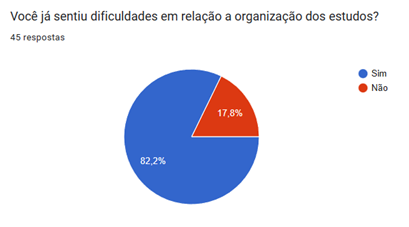
\includegraphics[width=12cm]{img1.png}
    Fonte: Os autores
    \label{fig01}
\end{figure}

Ao ser questionado, foi possível concluir que a quantidade de entrevistados que, em algum momento de sua experiência estudantil, já sentiram que precisavam de ajuda psicológica para lidar com a situação de pressão estudantil no \ac{IFSP} foi maior do que a quantidade de alunos que não sentiram a mesma necessidade (Figura~\ref{fig02}). 

\begin{figure}[H]
    \centering
    \caption{Necessidade de suporte psicológico para lidar com as pressões estudantis no IFSP}
    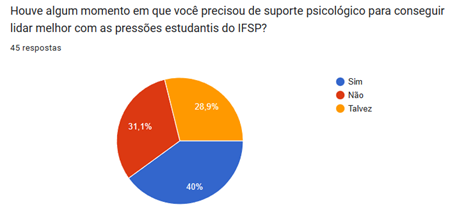
\includegraphics[width=14cm]{img2.png} \\
    Fonte: Os autores
    \label{fig02}
\end{figure}

Apesar de majoritariamente parte dos estudantes demonstrarem indiretamente carência de ferramentas proporcionadas por serviços assegurados pela \textit{Coordenadoria Técnico-Pedagógica (CTP)}, a grande maioria, isto é, 73,3\% dos discentes, nunca tentaram entrar em contato com a \ac{CTP} (Figura~\ref{fig03}).

\begin{figure}[H]
    \centering
    \caption{Entrevistados que tentaram entrar em contato com a CTP}
    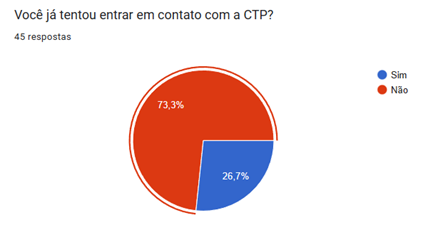
\includegraphics[width=12cm]{img3.png} \\
    Fonte: Os autores
    \label{fig03}
\end{figure}

O baixo índice de interesse no sentido de estabelecer contato com a \textit{Coordenadoria Técnico-Pedagógica (CTP)} pode ser explicado pela falta de divulgação da atuação do setor Sociopedagógico do Câmpus, bem como pela dificuldade encontrada por parte dos alunos na busca pelo serviço disponibilizado pela \ac{CTP}.

Após indagar dos estudantes o que eles estimavam de uma plataforma que tivesse o intuito de facilitar o contato entre o aluno e a \ac{CTP}, obteve-se que 86,7\% das respostas julgaram como uma plataforma necessária, enquanto apenas uma resposta foi contrária a ideia (Figura~\ref{fig04}).

\begin{figure}[H]
    \centering
    \caption{Entrevistados que consideram como necessária a criação da plataforma}
     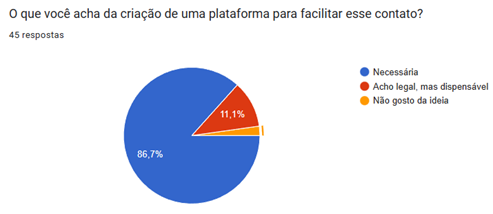
\includegraphics[width=15cm]{img4.png}
    Fonte: Os autores
    \label{fig04}
\end{figure}

Possuindo e analisando esses dados, faz-se importante a criação de um sistema (aplicação web) que facilite a comunicação entre o estudante do \ac{IFSP} e a \textit{Coordenadoria Técnico- Pedagógica (CTP)}, para que os alunos que apresentam alguma necessidade e sentem dificuldade de estabelecer contato ou entender o funcionamento do setor sejam auxiliados; além de organizar a demanda que chega para a \ac{CTP} em função dos processos e incidentes.

 Ademais, em ciência após diálogo com a \textit{Coordenadoria Técnico-Pedagógica (CTP)}, atualmente não chegam somente inquisições acerca de acompanhamentos psicológicos, mas também dúvidas gerais que geralmente são tratadas por outro setor e de outra forma, uma vez que a \ac{CTP} integra também a \textit{Diretoria adjunta Sociopedagógica}. Assim, igualmente se faz necessário, pois é capaz de organizar os processos que chegam para a \textit{Coordenadoria Técnico-Pedagógica (CTP)}, minando qualquer tipo de atraso ou confusão no momento de atender as exigências e estabelecer ordem de importância para tais. 

\subsection{Objetivo}

O projeto \gls{CTP Acolhe} tem como objetivo tornar mais fácil a comunicação direta entre os alunos e a \textit{CTP (Coordenadoria Técnico-Pedagógica)} do \ac{IFSP}, centralizando esses incidentes, ao mesmo tempo que divulga o seu apoio pedagógico e psicológico aos estudantes. 

Além disso, por meio de perguntas e respostas, a equipe fará uma coleta de informações iniciais importantes para caracterizar cada incidente, com o intuito de melhorar a organização desses incidentes por prioridades, de acordo com requisitos que estão sendo discutidos com a \ac{CTP} durante o desenvolvimento do projeto. 

Os integrantes da \gls{Lotus} também buscam passar confiança e segurança aos alunos que buscarem ajuda através do \gls{CTP Acolhe}, pois, ainda que seja normal precisar de ajuda, muitos alunos podem sentir medo de serem expostos ou se sentirem vulneráveis ao entrar em contato com a Coordenadoria Técnico-Pedagógica em busca de auxílio. 

\newpage

\section{Desenvolvimento}

\subsection{Divisão de tarefas}
As tarefas foram divididas de acordo com a área de interesse e competência de cada componente da \gls{Lotus}. Sendo assim, há uma grande distribuição de atividades visando melhorar o fluxo do desenvolvimento. Ademais  documentação fica a cargo de todos os elementos da equipe, por conta da interdisciplinaridade de cada ofício.

 O quadro da distribuição foi feito da seguinte forma (Figura~\ref{taf}):
\begin{figure}[H]
    \centering
    \caption{Cada área há um gerente ou mais para se responsabilizar quanto ao desenvolvimento de cada     parte do projeto.} 
     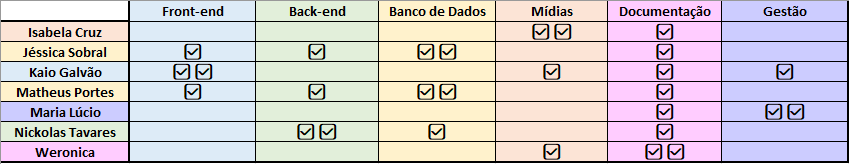
\includegraphics[width=15cm]{taf.png}
    Fonte: Os autores
    \label{taf}
\end{figure}

\subsection{Tecnologias e ferramentas}
Uma das etapas mais importantes no processo de desenvolvimento de um sistema é a escolha das tecnologias que vão ser utilizadas. Numa era com mudanças tão rápidas, principalmente no setor informático e tecnológico, é preciso que as escolhas sejam feitas com uma visão de longo prazo, na tentativa de acompanhar as tendências do mercado para que o produto não se torne ultrapassado em questão de poucos anos. Além do dilema da durabilidade das tecnologias escolhidas, estas também devem atender às necessidades do projeto, de forma que tudo o que se pretende fazer possa ser desenvolvido sem maiores dificuldades. Portanto, é essencial que uma análise o mais completa possível seja feita em relação ao mercado e às necessidades do projeto. Assim, estas foram as tecnologias escolhidas para o desenvolvimento deste projeto:

\begin{enumerate}
    \item Banco de dados
\begin{description}
    \item a) MySql: A princípio, a utilização do \gls{MySQL} era destinada a projetos de pequeno e médio porte, mas atualmente ele consegue suportar muito mais registros e processamentos. É um sistema de fácil emprego, com constantes atualizações, além de ser usado por empresas de renome que possuem um volume de dados gigante, tais como \gls{Bradesco}, \gls{Sony} e a própria \gls{NASA}. Por ser desenvolvido em \gls{C} e \gls{C++}, é compatível com diversos sistemas operacionais, a citar os mais importantes do mercado atualmente: \gls{Windows}, \gls{Linux} e \gls{Mac OS X Server}. Ele também possui interface para várias linguagens, incluindo as que serão utilizadas neste projeto; além de alta velocidade, uma já citada grande capacidade de execução e armazenamento, e utilização de \gls{SQL}, que é a linguagem mais utilizada quando se fala em banco de dados.   Ademais, ele é o segundo Sistema de Gerenciamento de Banco de Dados (SGBD) mais popular do mundo segundo o \gls{DB-Engines} , principal ranking do assunto; e o primeiro segundo a pesquisa “Tecnologias mais populares de 2022”, realizada pelo \gls{StackOverflow} . Outrossim, é uma ferramenta com a qual já se tem muita familiaridade.\cite{mysql}\\\\
\end{description}

    \item Back-End
\begin{description}
    \item a) Java: Criada pela  \textit{Sun Microsystems} e posteriormente adquirida pela \gls{Oracle}, o \gls{Java} tornou-se um gigante no desenvolvimento de aplicações. É uma linguagem orientada a objetos e tem como foco alta performance, portabilidade — pode ser o código pode ser escrito uma só vez e rodado em diversos dispositivos —, e segurança.  Além disso, o \gls{Spring}, framework\footnote{É uma estrutura que serve de base para a construção de aplicações web de finalidade específica} mais popular quando se fala de \gls{Java}, também será utilizado, visto que poupa tempo quando se fala de configuração e padronização, dando mais foco ao desenvolvedor para o desenvolvimento em si do que para a infraestrutura do projeto. Analisando o mercado, o Java está entre as dez linguagens de programação, scripting\footnote{É um código usado para otimizar processos em sistemas computacionais} e marcação mais populares segundo a pesquisa “Tecnologias mais populares de 2022”, já citada; e o \gls{Spring} está entre os cinco frameworks mais populares. O \gls{Java} e seu framework, Spring, já foram utilizados em projetos anteriores.\cite{java}\\
\end{description}

  \item Front-End
\begin{description}
   \item a) HTML: O HyperText Markup Language \ac{HTML} é uma linguagem de marcação vastamente utilizada no desenvolvimento web, tornando-se indispensável para qualquer projeto que siga este objetivo. É um dos pilares para a estruturação da interface do sistema, além de muito conhecida no mercado e pela equipe.\cite{html}\\

    \item b) CSS: O Cascading Style Sheets \ac{CSS} é uma linguagem de estilização, responsável pela personalização dos elementos marcados pelo \ac{HTML}: cores, fontes, tamanhos etc. são todos definidos por esta linguagem. Ademais, ela já está muito consolidada no mercado, tem uma facílima integração com as outras linguagens escolhidas e compõe a experiência da equipe.\cite{css}\\

\newpage

    \item c) JavaScript: Ao lado do \ac{HTML} e do \ac{CSS}, o \gls{JavaScript} lidera o ranking de linguagens de programação, scripting e marcação da pesquisa já citada do \\ \gls{StackOverflow}, formando o trio de linguagens mais populares no desenvolvimento web atualmente. É uma linguagem de programação de alto nível intensamente utilizada para fornecer dinamicidade e interação de elementos dentro de uma página. Por fim, também já foi utilizada pela equipe em outros projetos.\cite{js}\\

    \item d) React.js: O React é uma biblioteca JavaScript que possibilita que certos elementos de uma página possam ser separados em componentes reutilizáveis. Assim sendo, um botão pode ser desenvolvido uma única vez para ser utilizado em inúmeras páginas do mesmo projeto. Além disso, ele fornece mais dinamicidade ainda à interface, graças à sua administração de estado, que permite que algumas informações sejam passadas entre diversos componentes para suas respectivas atualizações apenas se for necessário, não havendo necessidade de atualizar a página inteira. Criada em 2011 pelo \gls{Facebook}, o React hoje, segundo o \gls{StackOverflow}, está entre as principais tecnologias web, perdendo apenas para o Node.js. Alguns membros da equipe já utilizaram esta tecnologia e conhecem seu funcionamento.\cite{react}\\
\end{description}

    \item Versionamento
    \begin{description}
        \item a) SubVersion: O \textit{SubVersion  (SVN)} é um controlador de versão que gerencia arquivos e diretórios, tornando possível visualizar o histórico de alterações, os autores dessas alterações e sua recuperação. É muito proveitoso para trabalhar em grupo, visto que muitos usuários podem fazer suas modificações sempre que necessário. Esta ferramenta foi escolhida porque é uma obrigatoriedade da matéria de PDS.\cite{svn}\\
    \end{description}

    \item Documentação
    \begin{description}
        \item a) \LaTeX: O \LaTeX  é um sistema de composição que permite que documentos sejam criados num formato predeterminado sem que haja grandes dificuldades de configuração. Para tanto, a equipe optou por utilizar o \gls{Overleaf}, que permite a criação de documentos, relatórios, projetos etc. a partir do emprego do \LaTeX. Esta ferramenta também foi escolhida por ser uma obrigatoriedade da matéria de \ac{PDS}, além de permitir que todos os integrantes tenham acesso à edição do mesmo documento.\cite{latex} 
    \end{description}
\end{enumerate}

\newpage

\subsection{Arquitetura de software}
Por se tratar de uma aplicação web, uma discussão principal durante o processo criativo inicial do projeto foi de escolher não apenas um padrão de desenvolvimento apropriado, mas também uma arquitetura escalável e flexível.

Para isso, adotou-se a arquitetura de sistema \gls{REST API} \cite{api} a fim de tornar o desenvolvimento do \gls{Front-end} e \gls{Back-end} independentes, adotando um modelo cliente-servidor, no qual o cliente envia requisições \gls{HTTP} e o servidor fornece as respostas correspondentes representadas, no caso do projeto \gls{CTP Acolhe}, em \gls{JSON} \cite{json}. Uma vez que estruturado, esse modelo garante não somente que o sistema tenha escalabilidade e portabilidade em várias plataformas, mas também torna a revisão de código mais prática a longo prazo, evitando que o sistema se torne \gls{hard-code} \cite{hard}.

Nesse sentido, \gls{Railway} foi a plataforma designada para hospedar tanto o banco de dados quanto o back-end do projeto, dado que é gratuita para uso moderado e descomplica a integração do banco de dados com a \gls{API}.
Apropriado ao front-end, optou-se pelo \gls{Netlify} \cite{netlify} como solução de hospedagem, visto que oferece certificado \gls{TLS} 1.3 \cite{tls} gratuito e recursos de \gls{CDN} \cite{cdn} que melhoram a velocidade de carregamento de página, além de permitir deploy para mais de uma branch, o que proporciona testes em ambiente concreto.

Ambas as plataformas de hospedagem foram escolhidas posto que oferecem integração com repositórios \gls{Git} \cite{git}, como o \gls{GitHub} \cite{gith} – local onde ocorre o versionamento da aplicação, facilitando o processo de deploy contínuo. 
Por fim, para o banco de imagens, está sendo utilizado temporariamente o \gls{Discord}. Porém, a perspectiva é adotar o \gls{imgBB}, justamente por ser um serviço de hospedagem gratuito que fornece recursos que se espera de um serviço de armazenamento de imagens, como interpretar as imagens em links por exemplo, e principalmente pelo recurso de upload de imagens por meio de requisições na sua \gls{API}. \cite{arquitetura} (Figura~\ref{aqr}) 

\begin{figure}[H]
    \centering
    \caption{Arquitetura CTP Acolhe}
     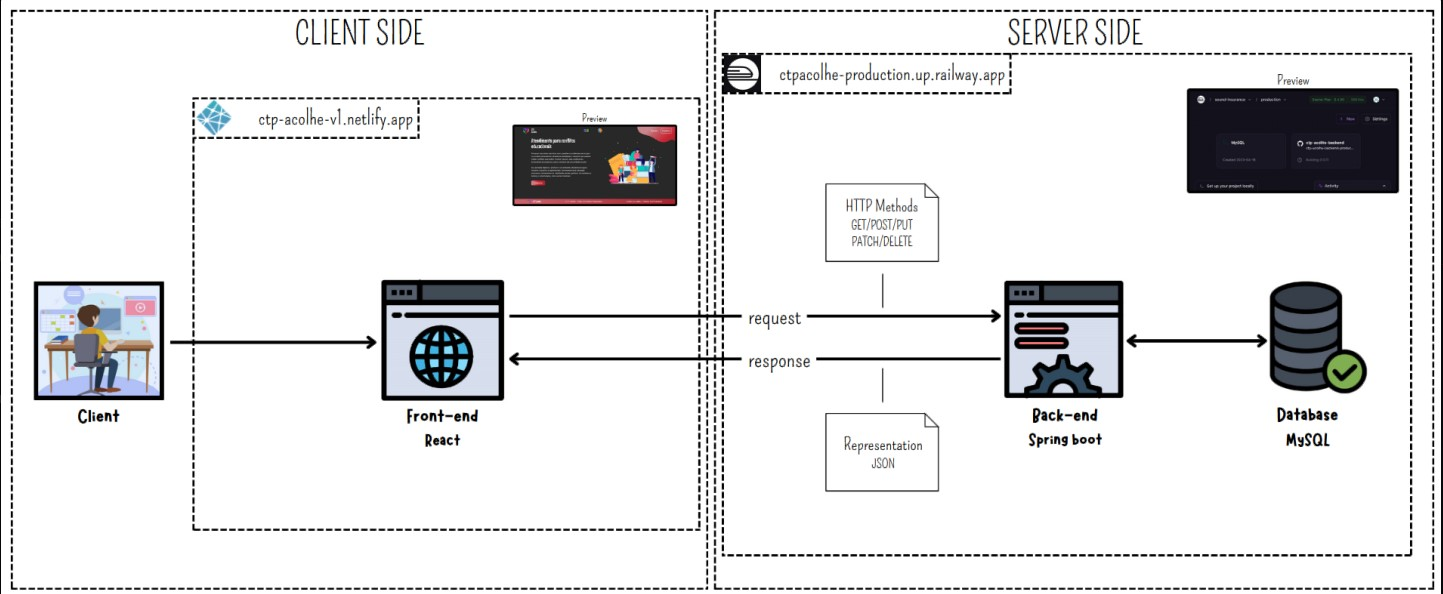
\includegraphics[width=15cm]{aqr.jpg} \\
    Fonte: Os autores
    \label{aqr}
\end{figure}

\newpage

\subsection{Análise de Requisitos}
A análise de requisitos visa identificar e definir as necessidades que o usuário espera sanar com o sistema que será desenvolvido, além de permitir explicitar as funcionalidades, permissões e as restrições do projeto. Desse modo, foi realizado pela equipe o levantamento dos Requisitos Não Funcionais \ac{RNF}, Requisitos Funcionais \ac{RF} e as Regras de Negócio \ac{RN}. \cite{vverner, mestres, artigoo} 

\subsection{Requisitos Não Funcionais (RNF)}
Os Requisitos Não Funcionais são aqueles que tratam dos atributos de qualidade que o sistema deve possuir como um todo, e não das funcionalidades específicas que são oferecidas por esse sistema. Visto a importância desse levantamento, foi-se realizado na (Figura~\ref{fig05}), listando os Requisitos Não Funcionais para o projeto \gls{CTP Acolhe}: (Figura~\ref{fig05}). \cite{artigo, blog, codificar}

\begin{figure}[H]
    \centering
    \caption{Descrição de requisitos não funcionais}
     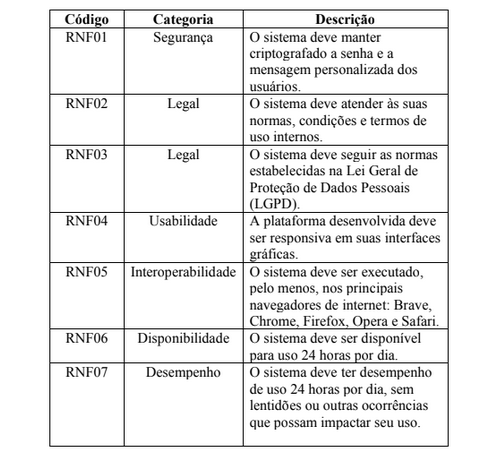
\includegraphics[width=13cm]{img05.png} \\
    Fonte: Os autores
    \label{fig05}
\end{figure}

\newpage

\subsection{Requisitos Funcionais (RF)}
Os Requisitos Funcionais são aqueles que especificam as funções e comportamentos que o sistema deverá seguir para atender às expectativas do usuário. É ideal que se defina o nível de prioridade para cada um desses requisitos a fim de definir sua importância e o esforço necessário para sua realização. Portanto, visando as principais funcionalidades do sistema, a equipe classificou os Requisitos Funcionais \cite{codificar}, em Alta, Média e Baixa prioridade: (Figura~\ref{o6})

\begin{figure}[H]
    \centering
    \caption{Descrição de requisitos funcionais}
     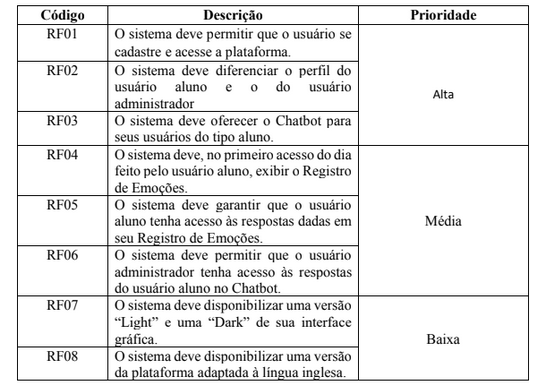
\includegraphics[width=15cm]{img6.png}
    Fonte: Os autores
    \label{o6}
\end{figure}

\subsection{Regras de Negócio (RN)}
As regras de negócio são um conjunto de declarações explícitas que definem como um negócio opera e quais são suas especificações. Essas declarações descrevem políticas, procedimentos, valores e restrições do negócio.

Segundo Dallavalle e Cazarini (2000), as Regras de Negócio são fundamentais pois afetam diretamente os requisitos funcionais do sistema; uma vez que, são regras do domínio de aplicação que devem ser tratadas no desenvolvimento.
Portanto, depreende-se que devem ser levantadas e documentadas de forma clara e objetiva, de modo a garantir com que todos compreendam as especificações do negócio. \cite{artigoo}

A documentação das regras de negócio envolve várias formas de representação e a escolha da melhor forma de fazê-la depende da complexidade do negócio e das necessidades do planejamento e dos \gls{Stakeholders}. Nesse sentido, para definir as regras de negócio, foi realizado a (Figura~\ref{p1}) que dispõe as Regras de Negócio do projeto \gls{CTP Acolhe}. \cite{artigoo}

\begin{figure}[H]
    \centering
    \caption{Regras de Negócio}
     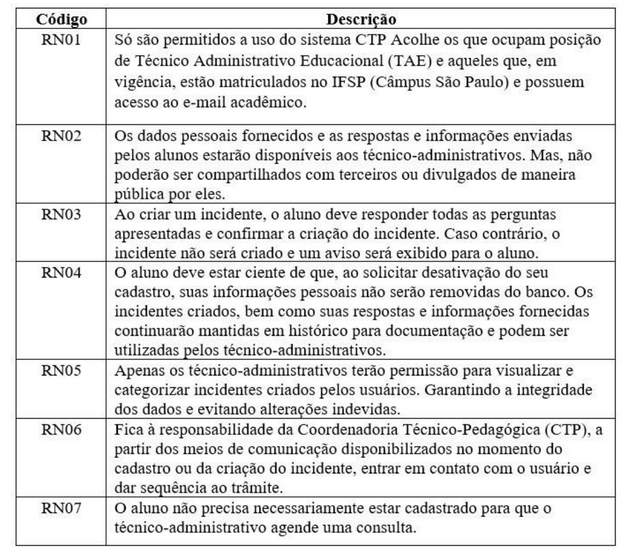
\includegraphics[width=15cm]{img8.png}
    Fonte: Os autores
    \label{p1}
\end{figure}

\newpage

\section{Modelagem}
\subsection{Diagrma de Casos de Uso}
\begin{figure}[H]
    \centering
    \caption{Caso de Uso}
     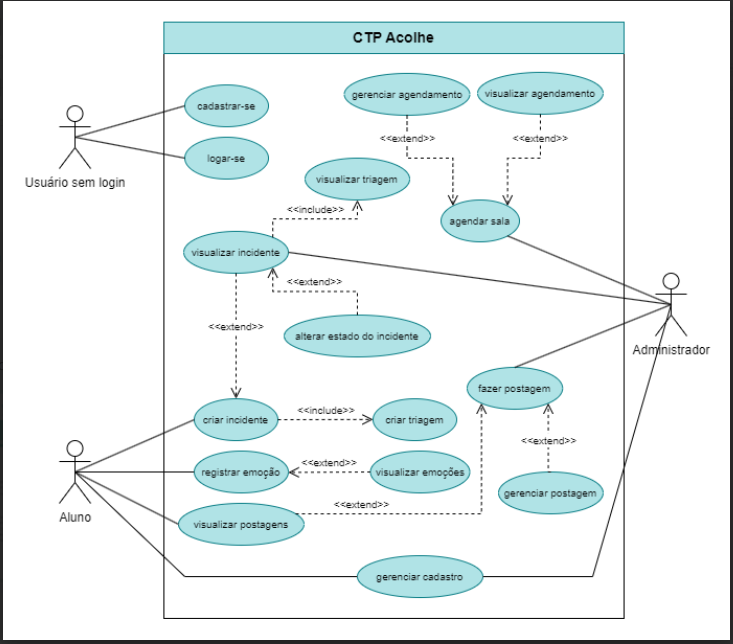
\includegraphics[width=15cm]{casouso.png}
     Fonte: Os autores
     \label{casouso}
\end{figure}

\newpage

\subsection{Diagrma de Classes}
O diagrama de classes tem como responsabilidade mapear e especificar as classes de determinado sistema com seus respectivos atributos e métodos, além do relacionamento entre objetos \cite{sig}. O diagrama feito para compor a documentação do projeto \gls{CTP Acolhe} foi feito tomando como base as classes a nível de entidade, isto é, aquelas que fazem conexão direta com o banco de dados a partir de um framework de permanência. Apesar de ser muito bem projetado e seguir lado a lado com a estrutura esperada no banco de dados, o diagrama pode sofrer algumas modificações ao longo do processo de desenvolvimento conforme alterações inesperadas ocorram. Assim, concluiu-se no esquema visualizável na  (Figura~\ref{dia}).

\newpage

\begin{figure}[H]
    \centering
    \caption{Diagrama de Classe}
     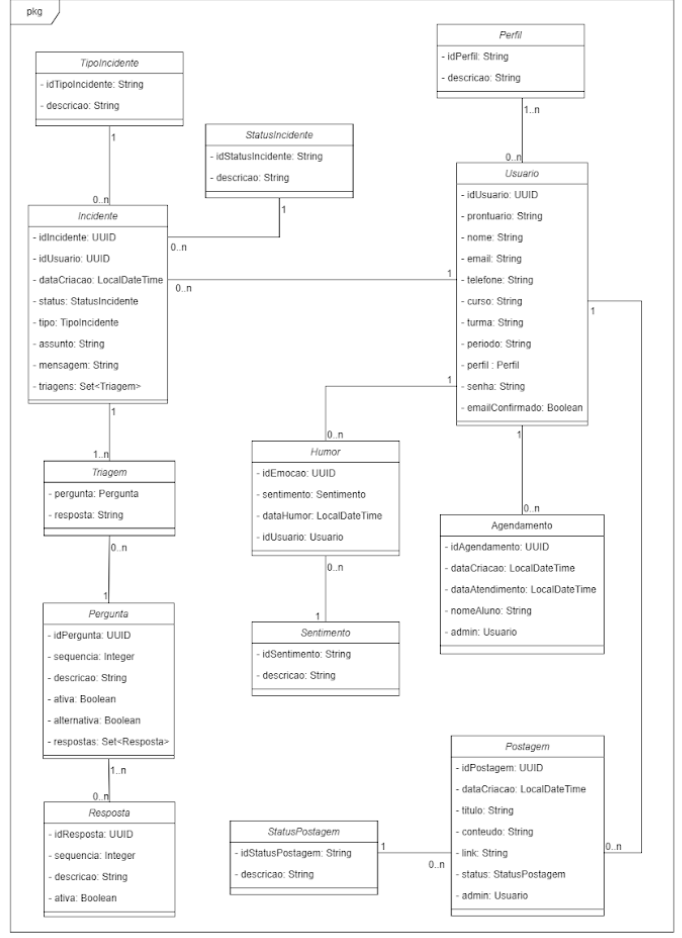
\includegraphics[width=15cm]{diagram.png}
    Fonte: Os autores
    \label{dia}
\end{figure}

\newpage

\subsection{Diagrama de Tabelas Relacionais (MER)}
Para aprofundar melhor, optamos pelo diagrama de tabelas relacionais, que é basicamente um diagrama de entidade-relacionamento \cite{luci}. Entretanto, neste é muito mais fácil visualizar como as tabelas do banco de dados e seus relacionamentos vão ficar na prática, isto é, já desenvolvidas. Também dá para colocar os tipos de dados dos atributos e a representação lógica das tabelas de relacionamento ou tabelas de entidades associativas, como dá para ver na (Figura~\ref{mer}).

\begin{figure}[H]
    \centering
    \caption{Diagrama de Tabelas Relacionais}
     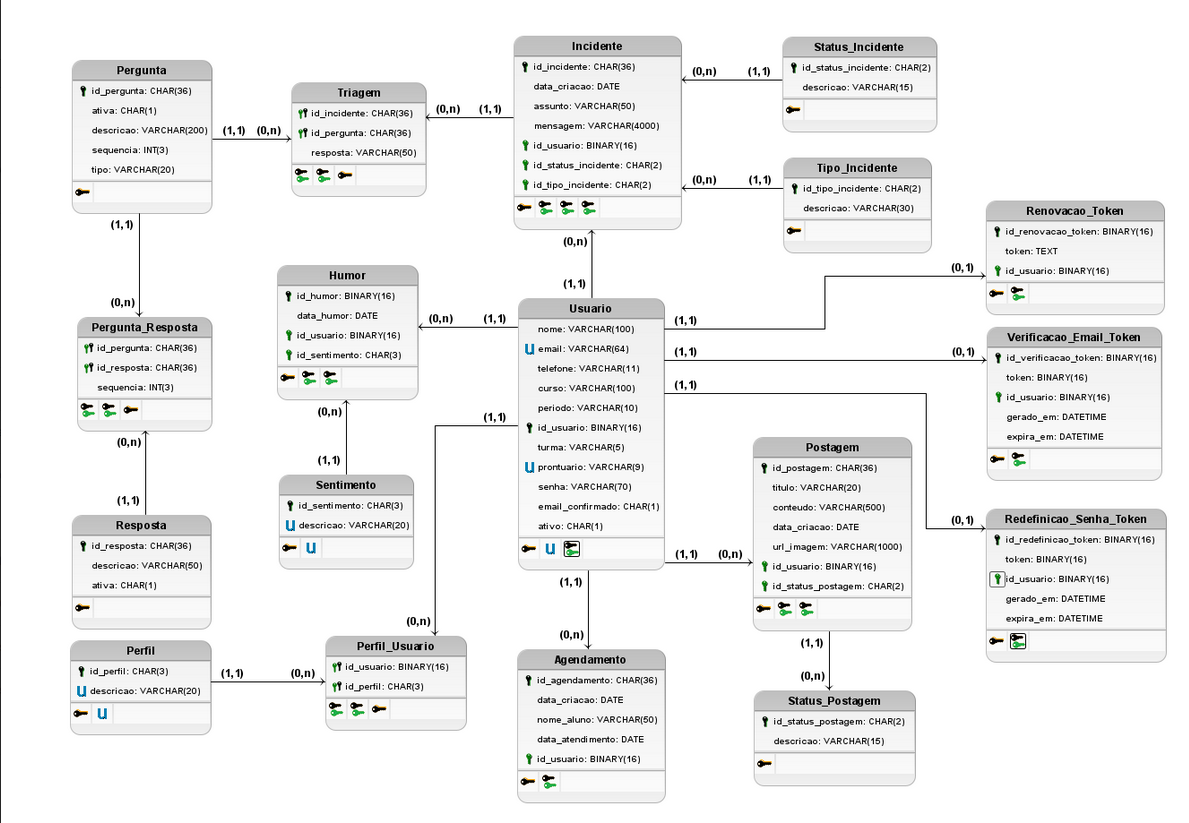
\includegraphics[width=15cm]{mer.png}
    Fonte: Os autores
    \label{mer}
\end{figure}

\newpage

\thispagestyle{plain}
\titleformat{\section}{\Centering\large\bfseries}{}{0.0px}{}
\phantomsection
\addcontentsline{toc}{section}{Referências}
{\bibliographystyle{plain}}
%\bibliographystyle{abntex2-alf}
\bibliography{sbc-template}

\newpage
\thispagestyle{plain}
\addcontentsline{toc}{section}{Glossário}
\thispagestyle{plain}
\printglossary

\newpage

\appendix
\thispagestyle{plain}
\addcontentsline{toc}{section}{Apêndices}
\section*{Apêndices}
\section{Apêndice A - Pesquisa de campo}

\begin{figure}[H]
    \centering
    \caption{Pesquisa de campo}
     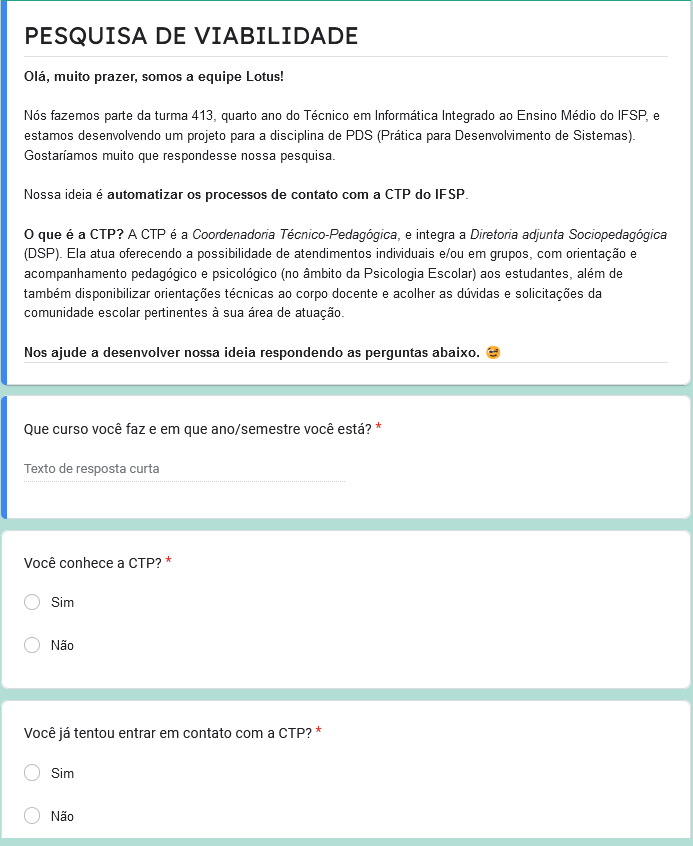
\includegraphics[width=15cm]{foto1.png}
\end{figure}

\newpage

\begin{figure}[H]
    \centering
     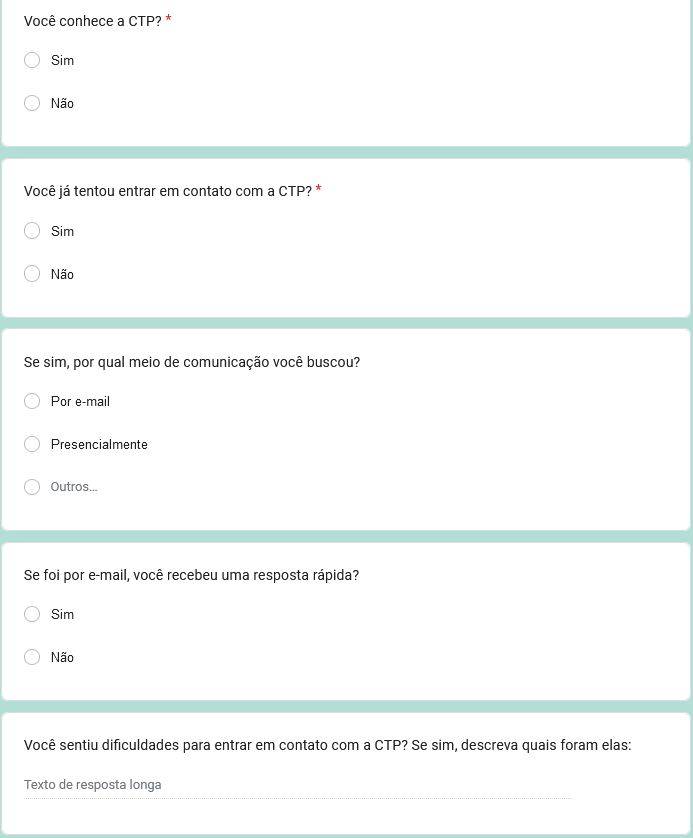
\includegraphics[width=15cm]{foto2.png}
\end{figure}

\begin{figure}[H]
    \centering
     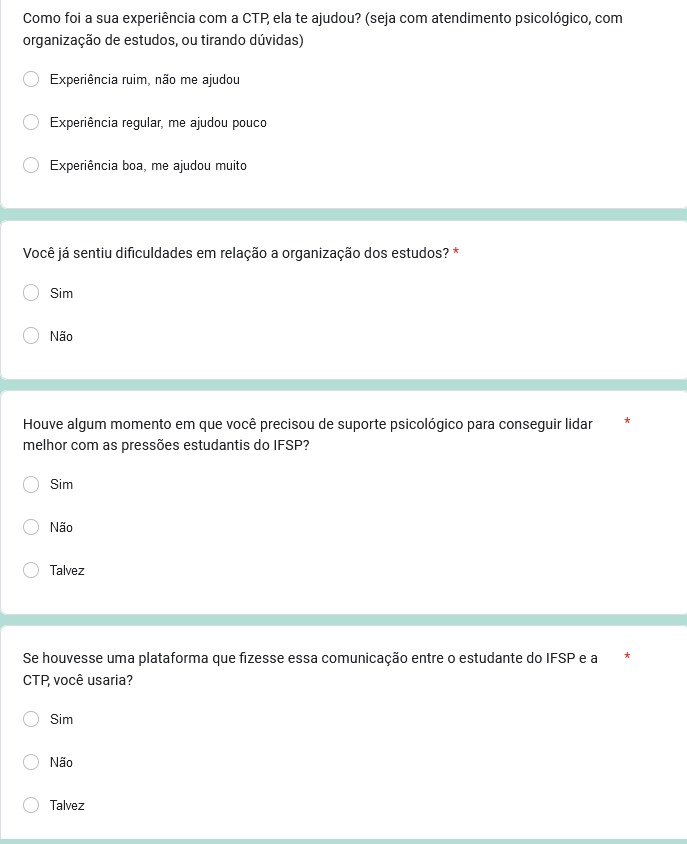
\includegraphics[width=15cm]{foto3.png}
\end{figure}

\begin{figure}[H]
    \centering
     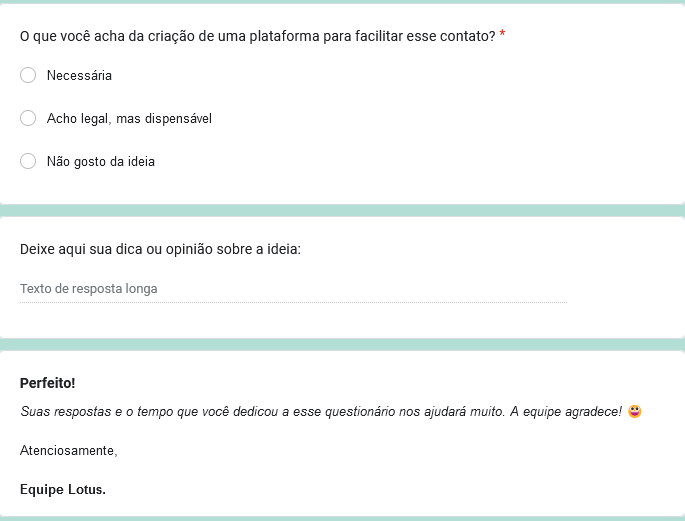
\includegraphics[width=15cm]{foto4.png}
     Fonte: Os autores
     \label{fig06}
\end{figure}

\newpage

\section{Apêncide B - Métodos de Gestão}
Para garantir que a organização do projeto, a definição de tarefas, os prazos de entrega e o desenvolvimento do sistema ocorram de forma eficaz, saudável e ágil para todos os membros da equipe, foram adotada metodologias ágeis que auxiliam a produtividade e a entrega de bons resultados no projeto.

Dentre as diversas metodologias ágeis, a equipe optou por selecionar o modelo \gls{Scrum}, pois é voltado para a gestão e planejamento de projetos de \gls{Software} e se enquadra nas necessidades que o projeto demanda. No entanto, houve adaptações nos padrões dessa metodologia para que sua aplicação fosse viável:

\begin{itemize}
    \item \textbf{Sprint:} Ciclos de atividades que foram adaptadas para durarem até duas semanas, devido às entregas frequentes que são exigidas pela disciplina;\cite{roberto}
    \item \textbf {Time-Boxed:} Tempo estipulado para que as atividades da Sprint sejam cumpridas, e que pode ser adaptado conforme a disponibilidade dos membros da equipe e por sua data de entrega;\cite{roberto}
    \item \textbf{Planejamento de Sprint:} Reuniões realizadas no início de cada ciclo para priorizar, definir como será feito e destituir as tarefas entre a equipe. Tais reuniões ocorrerão no dia seguinte ao fim da Sprint anterior e durarão cerca de 2 horas; \cite{roberto}
    \item \textbf{Reuniões diárias:} Não sendo possível realizar reuniões diárias de forma síncrona, a equipe optou por, diariamente, manter a comunicação sobre o desenvolvimento de cada tarefa de forma assíncrona, através dos canais de comunicação como WhatsApp ou Discord; \cite{roberto}
    \item \textbf{Revisão da Sprint:} A revisão da Sprint ocorrerá durante todo o seu desenvolvimento, seja nas aulas da disciplina de PDS, em atendimento aos alunos ou nas reuniões com a CTP, para que, assim, haja um feedback mais rápido sobre as melhorias do que está sendo desenvolvido; \cite{roberto}
    \item \textbf{Retrospectiva da Sprint:} Reunião feita no fim de cada Sprint, com duração de, aproximadamente, 2 horas e que aponta as dificuldades e ajustes encontrados na realização desse ciclo para que, dessa forma, a produtividade seja melhor na próxima Sprint. \cite{roberto}
\end{itemize}

Além da utilização do \gls{Scrum}, o quadro \gls{Kanban} foi escolhido pela equipe para a organização visual das \gls{Sprints}. O quadro em questão apresenta 5 colunas, que dispõem visualmente o estágio de cada tarefa, sendo elas “planejamento”, “a fazer”, “em andamento”, “revisão” e “concluído”. Além disso, cada tarefa possui uma data estipulada para entrega e também é classificada por ordem de prioridade, podendo ser “alta”, representada pela cor vermelha, “média”, representada pela cor amarela, ou “baixa”, representada pela cor verde. \cite{asana}

O quadro \gls{Kanban} foi desenvolvido na plataforma \gls{Trello}, permitindo que o mesmo seja compartilhado entre todos os membros da equipe e que seja acessado de qualquer lugar, para que todos possam fazer ajustes e ter total transparência sobre os itens desenvolvidos (Figura~\ref{l01}).

\begin{figure}[H]
    \centering
    \caption{Quadro de desenvolvimento de tarefas}
     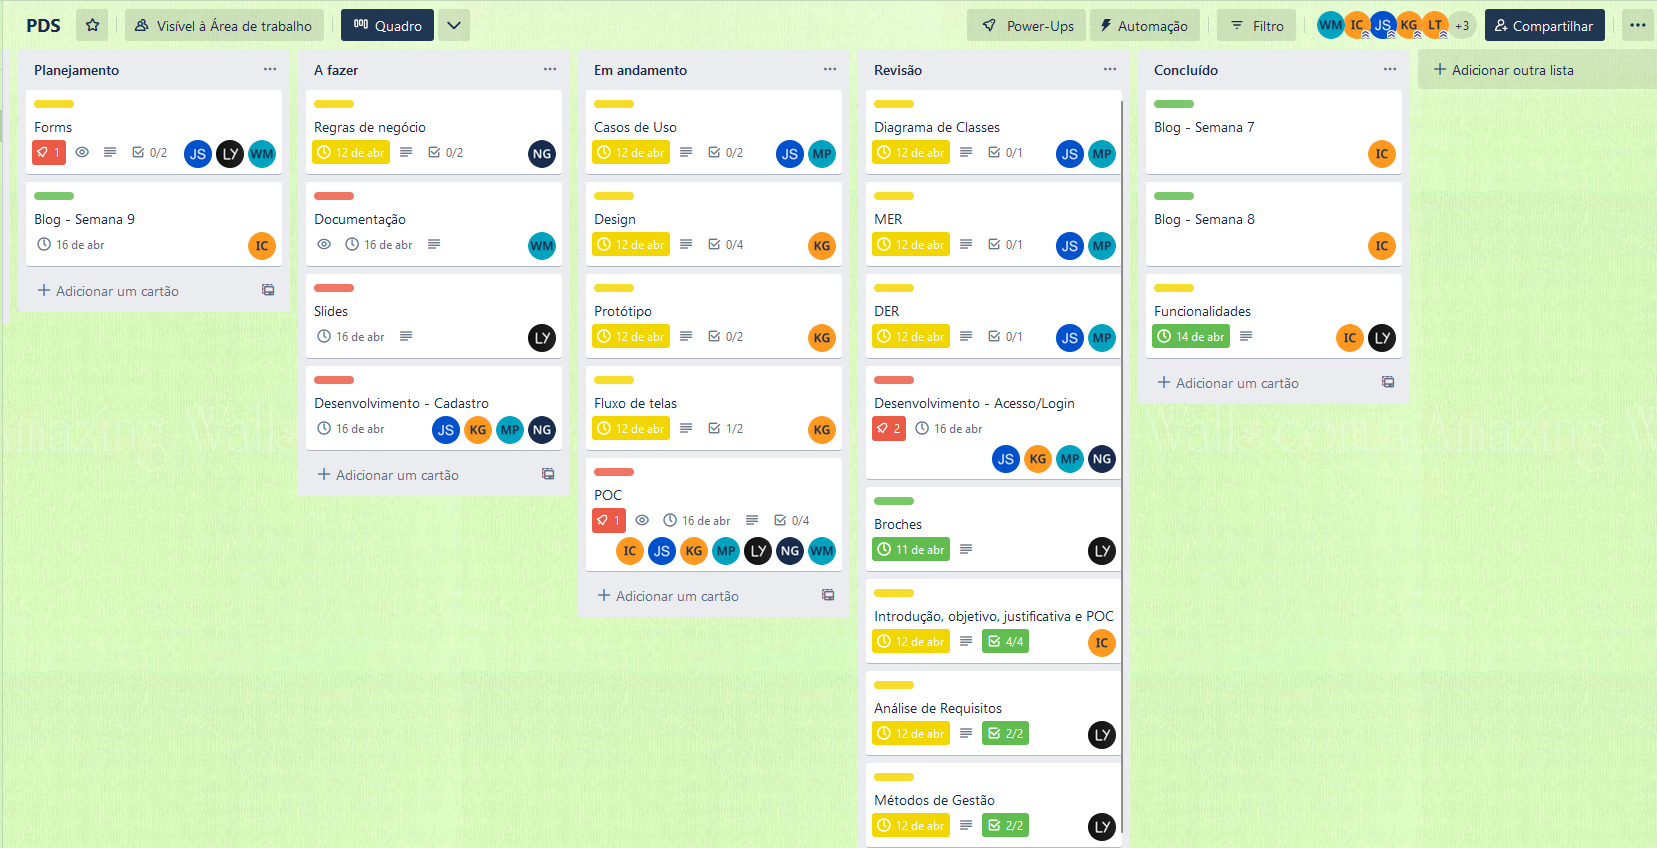
\includegraphics[width=15cm]{img7.png}
    Fonte: Os autores
    \label{l01}
\end{figure}

\newpage

\subsection{Diagrama Entidade Relacionamento (DER)}
O foco neste diagrama é especificar as entidades do banco de dados e seus relacionamentos entre si \cite{der}. Tradicionalmente, esse diagrama também apresenta os atributos das entidades, mas foi acordado que, como isso já é feito no diagrama de tabelas relacionais (Figura~\ref{mer}), não seria necessário. Portanto, essas são as entidades e os relacionamentos do sistema \gls{CTP Acolhe} (Figura~\ref{der}).

\begin{figure}[H]
    \centering
    \caption{Diagrama Entidade Relacionamento}
     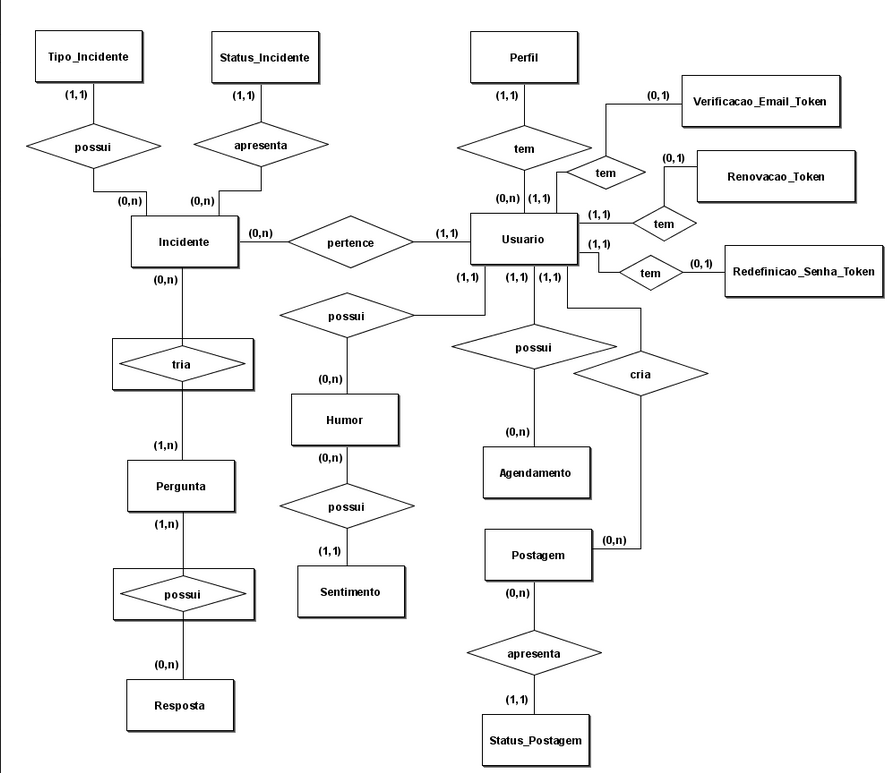
\includegraphics[width=15cm]{der.png}
    Fonte: Os autores
    \label{der}
\end{figure}

\newpage

\section{Apêndice C - Designe}
\subsection{Logo do Sistema/Aplicação}
Com o escopo do projeto definido, a próxima etapa da equipe foi estipular uma marca que caracterizasse  a aplicação. 
Dessa forma, foi definida a seguinte logo para o sistema \gls{CTP Acolhe}: (Figura~\ref{ft01}).

\begin{figure}[H]
    \centering
    \caption{Logo}
     
\includegraphics[width=12cm]{ft.png} \\
    Fonte: Os autores
    \label{ft01}
\end{figure}

Logomarca essa que foi feita utilizando a ferramenta do \gls{FIGMA} e de um banco de imagens gratuito, o \gls{FreePik}. Com a Logo, já foram definidas as cores principais do sistema e a tipografia de fontes – auxiliando, assim, o desenvolvimento das etapas posteriores do projeto, como o desenvolvimento da UI e da UX \cite{aela}.

\subsection{UI/UX Designe}
\ac{UI} Design tem com enfoque a interface de um determinado sistema; já a \ac{UX} tem como objetivo a experiência final do usuário, envolvendo todo o caminho que ele faz na aplicação até encontrar seu objetivo (BrainBlog).
Assim, na próxima etapa do desenvolvimento do design da aplicação, o pensamento foi de que – desde o momento que o usuário entrasse pela primeira vez, até o momento que saísse – a aplicação propusesse uma experiência intuitiva enquanto estivesse sendo utilizada. E, por ser um sistema que é voltado para os estudantes e a Coordenadoria Técnico Pedagógica, a acessibilidade e o fácil acesso foram priorizados \cite{aela}.

\newpage

\section{Apêndice D - Protótipo e Fluxo de Telas}
Em primeira instância, o usuário irá acessar o sistema e será exibido para ele uma Land-Page de apresentação do sistema, juntamente de duas opções: acessar e cadastrar.

\begin{figure}[H]
    \centering
    \caption{Homepage}
     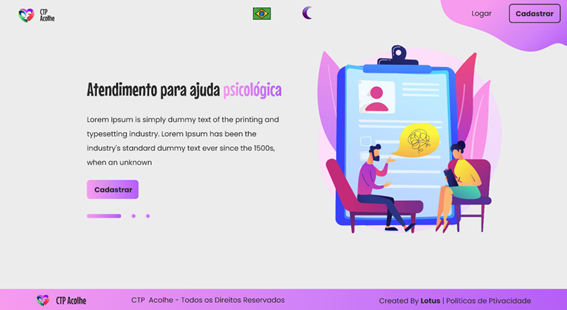
\includegraphics[width=15cm]{prot.png}
     Fonte: Os autores
\end{figure}

Há também a opção do usuário mudar a configuração de linguagem para inglês ou mudar o tema de \gls{Light} para \gls{Dark}. 

\newpage

\begin{itemize}
    \item \textbf{Mudança de Linguagem}
        \begin{figure}[H]
            \centering
            \caption{Homepage mudança de linguagem}
            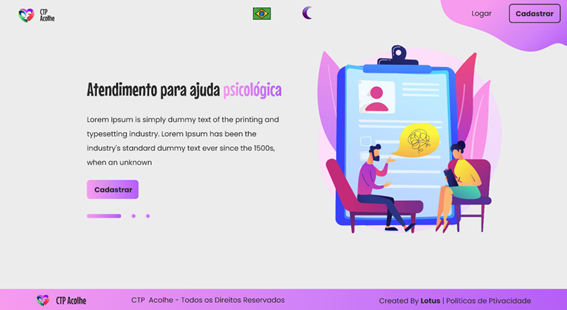
\includegraphics[width=15cm]{prot.png}
            Fonte: Os autores
        \end{figure}
    \item \textbf{Mudança de Tema}
        \begin{figure}[H]
            \centering
            \caption{Homepage mudança de tema}
            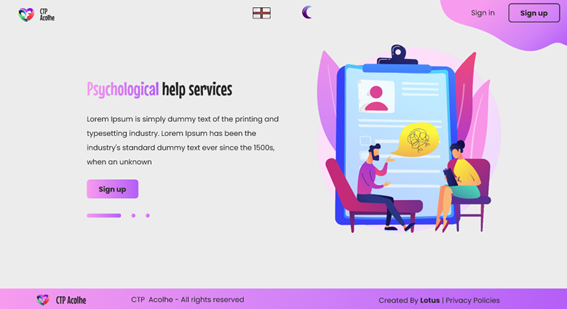
\includegraphics[width=15cm]{prot2.png}
            Fonte: Os autores
        \end{figure} 
\newpage
    \item \textbf{Land Page Slider}
        \begin{figure}[H]
            \centering
            \caption{Homepage slider}
            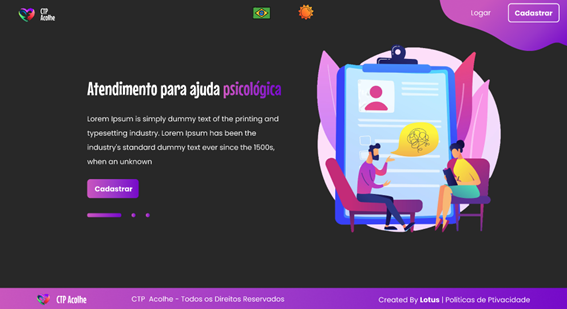
\includegraphics[width=15cm]{prot3.png}
            Fonte: Os autores
        \end{figure}
        \begin{figure}[H]
            \centering
            \caption{Homepage slider}
            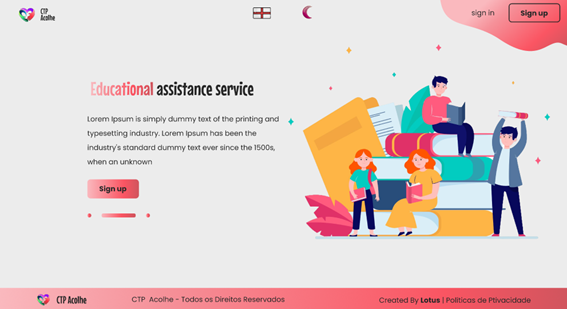
\includegraphics[width=15cm]{prot4.png}
            Fonte: Os autores
        \end{figure}
\newpage
        \begin{figure}[H]
            \centering
            \caption{Homepage slider}
            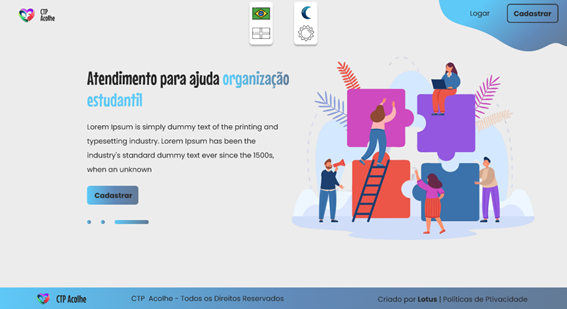
\includegraphics[width=15cm]{prot5.png}
            Fonte: Os autores
        \end{figure}
    \item \textbf{Login} \\ \\
    Caso o usuário já tenha uma conta no sistema, ele poderá clicar para fazer o login e será exibida a seguinte página:
        \begin{figure}[H]
                \centering
                \caption{Acessar}
                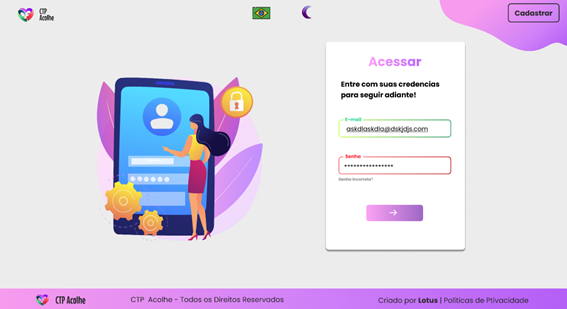
\includegraphics[width=15cm]{prot6.png}
                Fonte: Os autores
                \label{pt}
            \end{figure}
        Observe que ao preencher um campo corretamente, a borda do INPUT ficará verde, 
        \begin{figure}[H]
                \centering
                \caption{E-mail}
                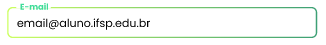
\includegraphics[width=15cm]{prot7.png}
                Fonte: Os autores
            \end{figure}
        enquanto quando se é preenchido de maneira incorreta, ficará vermelha.
         \begin{figure}[H]
                \centering
                \caption{Senha}
                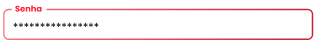
\includegraphics[width=15cm]{prot8.png}
                Fonte: Os autores
            \end{figure}
    
    \item \textbf{Registro de Emoçõe} \\ \\ 
    Após acessar a aplicação, o questionário de registro de emoções é feito ao usuário, na qual ele escolherá 1x por dia, nos dias que acessar, a emoção que mais condiz com o que está sentindo naquele dia. 
          \begin{figure}[H]
                    \centering
                    \caption{Antes da escolha}
                    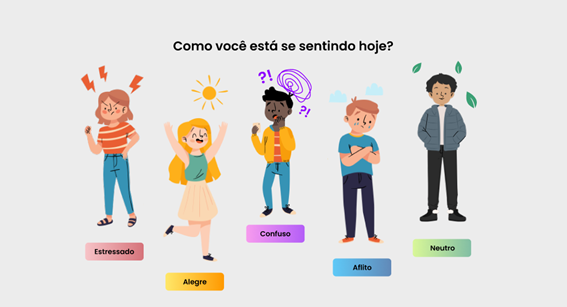
\includegraphics[width=15cm]{prot9.png}
                    Fonte: Os autores
                \end{figure}
            \begin{figure}[H]
                \centering
                \caption{Após a escolha}
                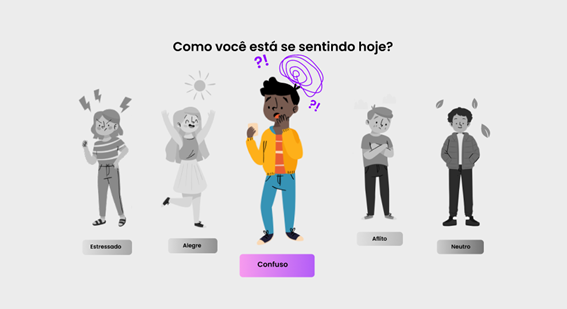
\includegraphics[width=15cm]{prot10.png}
            \end{figure} 
        Após o registro diário de emoção, o usuário tem acesso livre ao sistema e às demais funcionalidades que ele oferecerá, que estão em desenvolvimento. \\
    \item \textbf{Usuários sem cadastro} \\ \\
    Para aqueles que ainda não possuem cadastro no sistema, ao clicarem na opção de cadastrar, serão redirecionados para a página de cadastro, na qual poderão preencher os campos com suas informações, a fim de acessar o sistema.
            \begin{figure}[H]
                        \centering
                        \caption{Tela de cadastro}
                        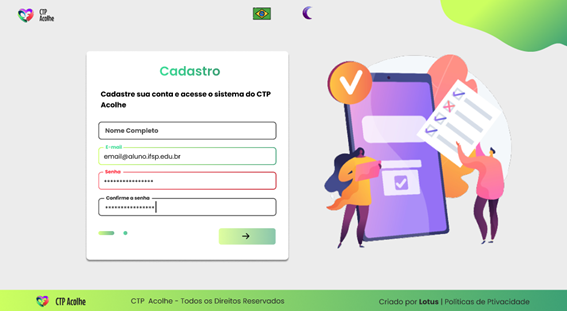
\includegraphics[width=15cm]{prot11.png}
                        Fonte: Os autores
                    \end{figure}  
        Observe que: \\
        1 - Quando o campo não foi preenchido, aparecerá a descrição dele no centro; 
             \begin{figure}[H]
                            \centering
                            \caption{Nome}
                            
\includegraphics[width=15cm]{prot12.png}
                            Fonte: Os autores
                        \end{figure} 
        2- Quando o campo preenchido for elegível, aparecerá uma borda verde; 
                \begin{figure}[H]
                                \centering
                                \caption{E-mail}
                                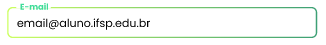
\includegraphics[width=15cm]{prot13.png}
                                Fonte: Os autores
                            \end{figure} 
        3 - Quando as informações não forem aceitas, a borda será vermelha; 
                \begin{figure}[H]
                                \centering
                                \caption{Senha}
                                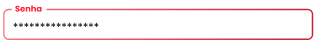
\includegraphics[width=15cm]{prot14.png}
                                Fonte: Os autores
                            \end{figure} 
        Enquanto o campo está sendo preenchido, a descrição ficará fixa à parte superior do input.
                 \begin{figure}[H]
                                \centering
                                \caption{Confirmação de senha}
                                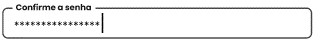
\includegraphics[width=15cm]{prot15.png}
                                Fonte: Os autores
                            \end{figure}
        Após realizar o cadastro, o usuário poderá acessar o sistema conforme a (Figura~\ref{pt}).
\end{itemize}

\newpage

\section{Apêndice E  - Atas de reuniões}
\begin{figure}[H]
    \centering
    \caption{Primeira reunião}
     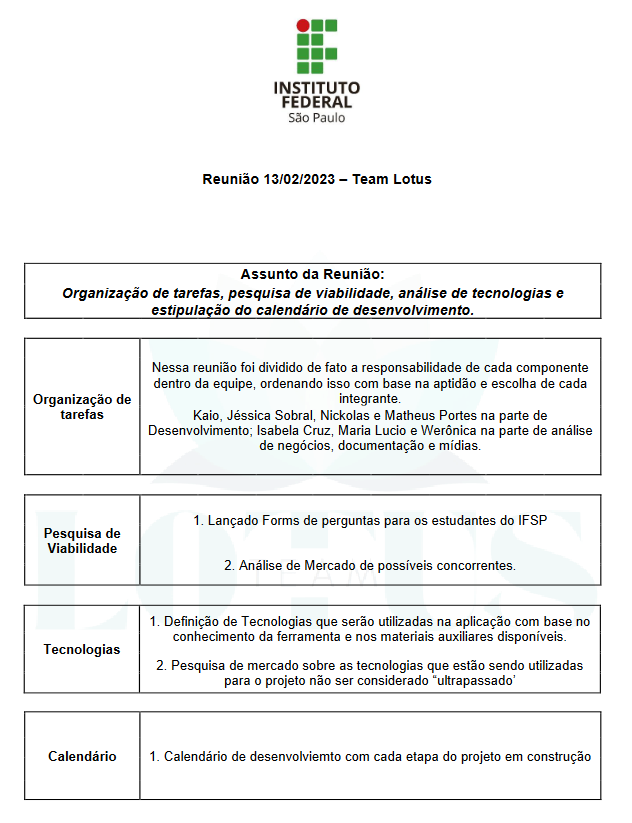
\includegraphics[width=15cm]{ilus1.png}
     Fonte: Os autores
     \label{fig07}
\end{figure}

\newpage

\begin{figure}[H]
    \centering
    \caption{Segunda reunião}
     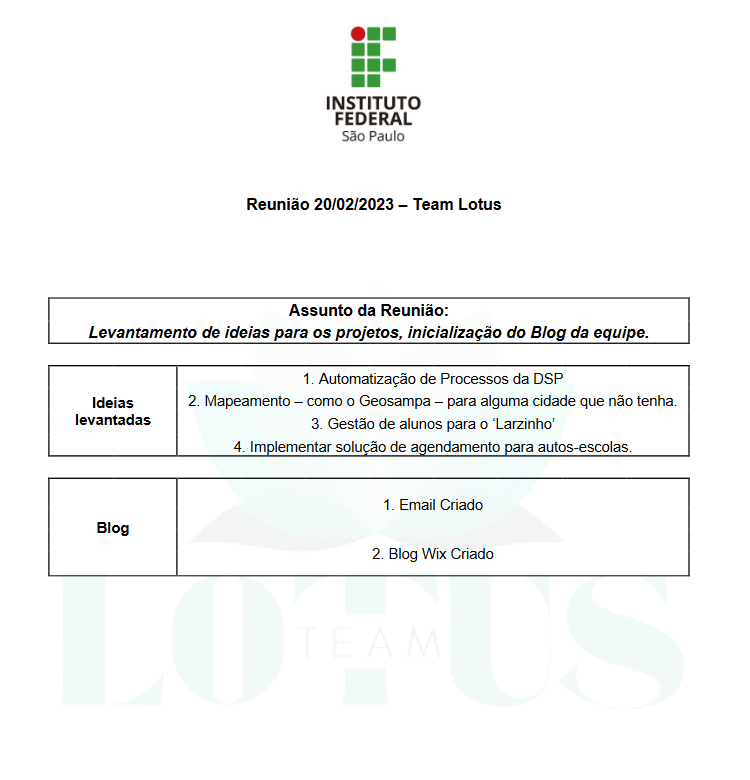
\includegraphics[width=15cm]{ilus2.png}
     Fonte: Os autores
     \label{fig08}
\end{figure}

\begin{figure}[H]
    \centering
    \caption{Terceira reunião}
     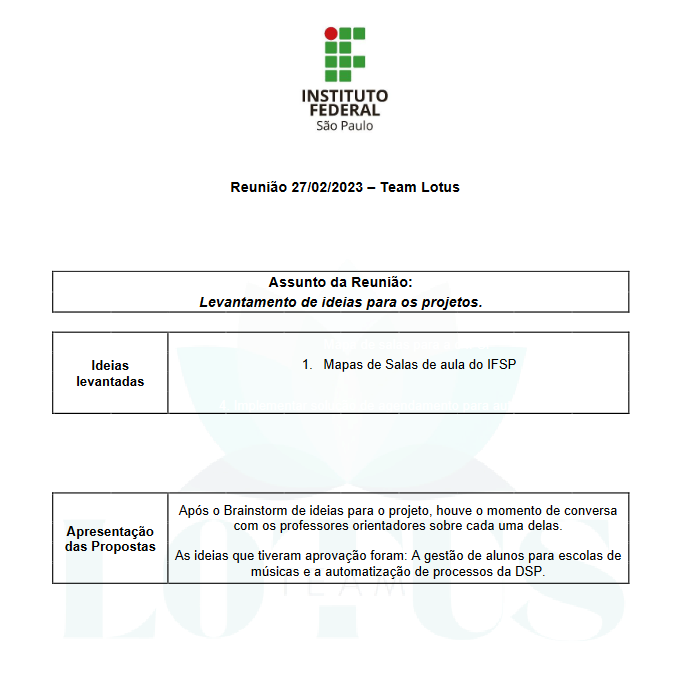
\includegraphics[width=15cm]{ilus3.png}
     Fonte: Os autores
     \label{fig09}
\end{figure}

\begin{figure}[H]
    \centering
    \caption{Quarta reunião}
     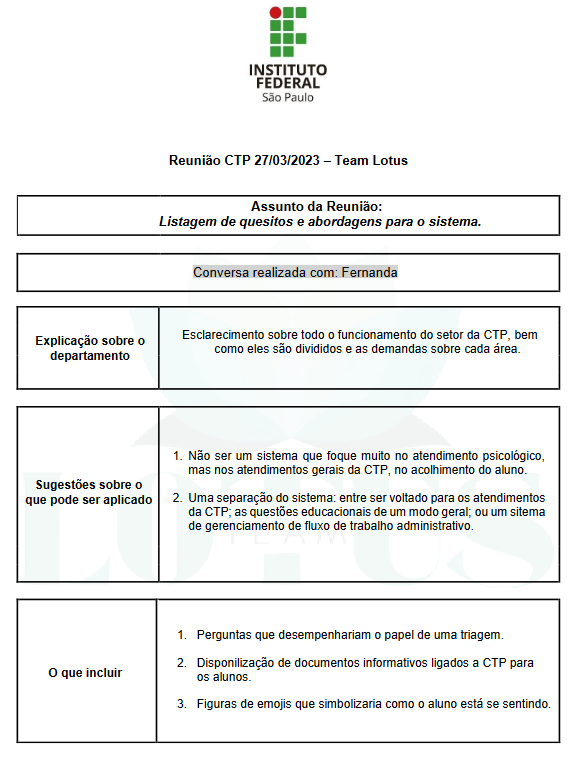
\includegraphics[width=15cm]{ilus4.png}
     Fonte: Os autores
     \label{fig}
\end{figure}

\begin{figure}[H]
    \centering
    \caption{Quinta reunião}
     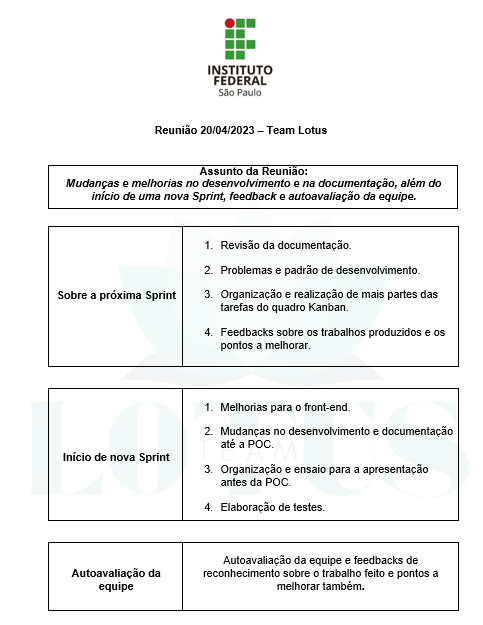
\includegraphics[width=15cm]{ilus5.png}
     Fonte: Os autores
     \label{ata}
\end{figure}

\newpage

\section{Apêndice F - Prova de Conceito}
O uso da Prova de Conceito possibilita a percepção e análise de uma aplicação com mais clareza, apresentado os riscos e a viabilidade da implementação. Através da realização da \ac{POC}, é possível colocar em prática as ideias que, até então, sáo apenas teorias, testando funcionalidades e observando se o projeto cumpre com aquilo que se propõe a fazer. 

O desenvolvimento funcionalidades principais de um projeto web através da \ac{POC} coloca a ideia geral em enquadramento, o que permite que a equipe faça uma análise mais completa de todo o projeto e suas tecnologias, e realize uma estrutura melhor para as demais ideias e funcionalidades. 

Para a realização de uma Prova de Conceito, existem alguns pontos que precisam ser levados em consideração. Em primeiro lugar, é preciso pensar qual é o objetivo dela, o que se pretende alcançar. Em segundo, é preciso pensar no que será testado, quais são as funcionalidades. Além disso, é importante levar em consideração o prazo e o tempo disponível para a realização da \ac{POC}. Ademais, se faz fundamental analisar os recursos e a equipe. Tendo as respostas dessas questões em mente, é possível produzir a Prova de Conceito \cite{gaspar} \cite{supero}.

\subsection{Prova de Conceito: CTP Acolhe}
A \ac{POC} do Projeto \gls{CTP Acolhe}, é formada por duas funcionalidades iniciais da aplicação, sendo elas: o cadastro na plataforma e o acesso do usuário. 

O \textbf{cadastro} pede ao usuário algumas informações, sendo elas: nome, e-mail, curso, período, turma, telefone, senha e confirmação de senha. Essas informações variam de acordo com o tipo de usuário, que pode ser do tipo aluno ou administrador — identificável pelo domínio do e-mail "@aluno.ifsp.edu.br" ou "@ifsp.edu.br".

O \textbf{acesso}, é dividido em dois tipos de usuários: do tipo aluno e do tipo administrador. Para realizar o acesso, é preciso fornecer o e-mail e senha. 

\end{document}

